% =====================================================================
% THIS FILE IS THE SOURCE. Edit it, then rebuild the PDF with:
%     bash tools/compile.sh Unit_06_Where_the_Data_Comes_From
% (run from the Course_Rewrite folder; it compiles twice and reports
%  page count, overfull boxes, and em dashes)
%
% Do not edit the PDF directly. Figures are the fig_*.pdf files in this
% folder, regenerated by tools/make_module*_slide_figs.py.
%
% Originally converted from the 15-module draft by a one-shot script now
% parked in tools/one_shot_generators/. Re-running those would discard
% anything you change here, so they are kept out of tools/ on purpose.
% =====================================================================
\documentclass[aspectratio=169]{beamer}
\usetheme{default}
\usefonttheme{professionalfonts}
\usepackage{amsmath, amssymb, amsfonts}
\usepackage{graphicx}
\usepackage{booktabs}
\usepackage{bm}
\usepackage{hyperref}

\mode<presentation> {
    \usetheme{Frankfurt}
    \usecolortheme{default}
}

\newcommand{\xbar}{\bar{x}}
\newcommand{\yhat}{\hat{y}}

\newenvironment{principle}[1]{\begin{block}{\textbf{Principle:} #1}}{\end{block}}
\newenvironment{trap}[1]{\begin{alertblock}{\textbf{Trap:} #1}}{\end{alertblock}}
\newenvironment{practice}[1]{\begin{exampleblock}{\textbf{In practice:} #1}}{\end{exampleblock}}
\newenvironment{interview}[1]{\begin{exampleblock}{\textbf{You may be asked:} #1}}{\end{exampleblock}}
\newenvironment{yourturn}[1]{%
  \setbeamercolor{block title}{fg=white,bg=orange!80!black}%
  \setbeamercolor{block body}{bg=orange!12}%
  \begin{block}{\textbf{Your turn:} #1}}{\end{block}}
\newenvironment{livedemo}[1]{%
  \setbeamercolor{block title}{fg=white,bg=teal!80!black}%
  \setbeamercolor{block body}{bg=teal!12}%
  \begin{block}{\textbf{Live demo:} #1}}{\end{block}}
\newenvironment{llmcheck}[1]{%
  \setbeamercolor{block title}{fg=white,bg=violet!75!black}%
  \setbeamercolor{block body}{bg=violet!10}%
  \begin{block}{\textbf{LLM check:} #1}}{\end{block}}

\title{Where the Data Comes From}
\subtitle{Unit 6: Sampling, Selection, and Missingness}
\author{Stat 220 \textbar{} Statistics for Data Science}
\date{}

\begin{document}

\begin{frame}
  \titlepage
\end{frame}

% ======================================================================
\section{Why}
% ======================================================================
\begin{frame}{Where this fits}
\begin{itemize}
  \item Every technique in this course assumes the data in front of you represents the thing you
        care about.
  \item That assumption is made \emph{before} any modeling, it is rarely checked, and no amount of
        later cleverness repairs it.
  \item This module is about the questions to ask before you fit anything: who is in this data, who
        is missing, and what was actually measured?
\end{itemize}
\begin{principle}{the data-generating process is part of the analysis}
An answer computed from the wrong population is not approximately right. It is confidently wrong,
with a small standard error attached.
\end{principle}
\end{frame}

\begin{frame}{Live experiment: three ways to sample this room}
\begin{livedemo}{estimate the same number three ways}
We want the average number of hours of sleep this class got last night.
\begin{enumerate}
  \item \textbf{Convenience:} the four people nearest the front, read your number aloud.
  \item \textbf{Volunteer:} anyone who wants to report, raise your hand. We take the first six.
  \item \textbf{Random:} I draw six student IDs at random. If your number comes up, you report.
\end{enumerate}
I record all three estimates on the board.
\end{livedemo}
\vspace{0.2em}
{\tiny\textit{Materials: none, but have the roster handy for the random draw. Time: 12 minutes.}}
\centering\small Then everyone reports, and we compute the truth. Three estimates, one right answer.
\end{frame}

\begin{frame}{Stay here while they report: predict the failures}
\begin{itemize}
  \item \textbf{Convenience} samples the front row, which is not a random slice of anything. Who
        sits in front is correlated with a lot.
  \item \textbf{Volunteers} are people with something to report: the person who slept three hours
        and the person who slept eleven both want to say so.
  \item \textbf{Random} will be off too, but only by sampling error, which we can quantify with a
        standard error.
\end{itemize}
\begin{principle}{the difference between the two kinds of wrong}
Random sampling gives error you can put a number on. Biased sampling gives error you cannot see,
cannot measure, and cannot shrink.
\end{principle}
\end{frame}

\begin{frame}{What this unit gives you}
\begin{columns}[T]
\begin{column}{0.5\textwidth}
\textbf{Things to know}
\begin{itemize}\small
  \item the difference between a population, a sampling frame, and a sample
  \item the main sampling designs and what each one buys you
  \item how selection bias arises, including survivorship and nonresponse
  \item why a large biased sample can be worse than a small random one
  \item what missing data does, and the three ways it can be missing
  \item why measurement choices are modeling choices
\end{itemize}
\end{column}
\begin{column}{0.5\textwidth}
\textbf{Mistakes to stop making}
\begin{itemize}\small
  \item treating sample size as evidence of representativeness
  \item studying only the survivors, winners, or responders
  \item dropping rows with missing values without asking why they are missing
  \item imputing the mean and then reporting the resulting tighter interval
  \item accepting a proxy variable as if it were the concept you meant
  \item quoting a margin of error that only accounts for sampling error
\end{itemize}
\end{column}
\end{columns}
\end{frame}

% ======================================================================
\section{Sampling}
% ======================================================================
\begin{frame}{Population, frame, sample}
\begin{itemize}
  \item \textbf{Population:} everyone you want to describe. All customers, all flights, all voters.
  \item \textbf{Sampling frame:} the list you can actually draw from. Your CRM, the phone book,
        people with app notifications enabled.
  \item \textbf{Sample:} who ended up in the data.
\end{itemize}
Bias enters at both arrows: frame does not match population (\textbf{undercoverage}), and sample
does not match frame (\textbf{nonresponse}).
\begin{principle}{name your frame out loud}
``Our customers'' usually means ``customers with an email on file who opened the message.'' Saying
the real frame is often enough to spot the problem.
\end{principle}
\end{frame}

\begin{frame}{Four designs worth knowing}
\begin{itemize}
  \item \textbf{Simple random sample:} everyone equally likely. The benchmark.
  \item \textbf{Stratified:} split into groups (region, plan tier), sample within each. More
        precision for the same cost, and guarantees small groups appear.
  \item \textbf{Cluster:} sample whole groups (stores, classrooms) and measure everyone inside.
        Cheaper, but the effective sample size is closer to the number of clusters.
  \item \textbf{Systematic:} take every $k$th record. Fine unless the list has a hidden periodicity.
\end{itemize}
\begin{trap}{cluster samples analyzed as if they were random}
Surveying 20 stores with 50 customers each is not 1{,}000 independent observations. Treating it as
such is the standard-error error from the CLT module, at scale.
\end{trap}
\end{frame}

\begin{frame}{Survivorship bias: the most famous example}
\begin{center}
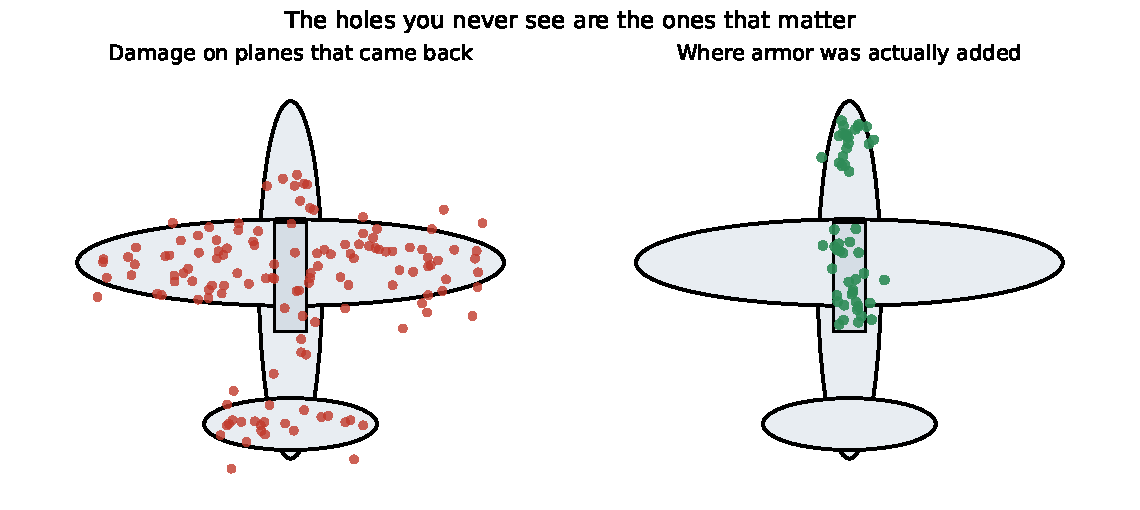
\includegraphics[width=0.84\textwidth]{fig_m14_survivorship.pdf}
\end{center}
\vspace{-0.4em}
\small
In World War II, analysts studied bullet holes in returning bombers and proposed armoring the
wings, where the holes were. Abraham Wald pointed out the obvious once you see it: those planes
came back. Armor belongs where the returning planes have \emph{no} holes, because planes hit there
did not return.
\end{frame}

\begin{frame}{Survivorship bias in business advice}
\begin{itemize}
  \item ``Five habits of successful founders'' studies only successful founders. The failed ones
        may have had the same five habits.
  \item Backtested trading strategies use indexes that quietly dropped delisted companies, so the
        historical return is measured only on the survivors.
  \item ``Our power users love this feature'' is measured among people who stayed. The ones the
        feature drove away are not in the data to complain.
\end{itemize}
\begin{practice}{how to spot it in one question}
``Who is missing from this dataset because of the outcome we are studying?'' If the answer is
``anyone,'' the analysis needs rework.
\end{practice}
\end{frame}

\begin{frame}{Nonresponse: the modern polling problem}
\begin{columns}[c]
\begin{column}{0.58\textwidth}
\centering
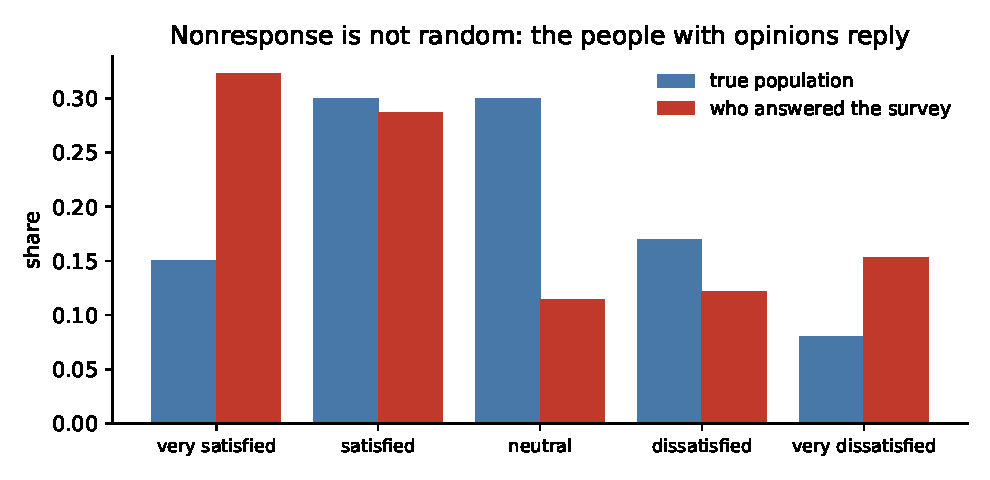
\includegraphics[width=\textwidth]{fig_m14_nonresponse.pdf}
\end{column}
\begin{column}{0.42\textwidth}
\small
People with strong feelings answer surveys. The indifferent middle does not.
\begin{itemize}
  \item Your satisfaction data becomes bimodal even when the population is not.
  \item Response rates for phone polls have fallen from over 30\% to under 10\%, and the tilt is
        what makes modern polling hard.
\end{itemize}
\end{column}
\end{columns}
\onslide<2->{\centering\small
Weighting can correct for \emph{measured} differences. It cannot correct for people who differ in
ways you did not record.}
\end{frame}

\begin{frame}{Two famous failures worth remembering}
\begin{itemize}
  \item \textbf{1936:} the \emph{Literary Digest} mailed 10 million ballots and got 2.4 million
        back, predicting a Landon landslide. Roosevelt won 46 states. The frame came from car and
        telephone registries in the Depression, and only the enthusiastic mailed back.
  \item At the same time George Gallup polled about 50{,}000 people, chosen to match the
        population, and got it right.
  \item \textbf{The lesson repeats:} 2.4 million biased responses lost to 50{,}000 designed ones.
\end{itemize}
\begin{principle}{design beats volume}
Sampling error shrinks with $n$. Sampling bias does not shrink at all.
\end{principle}
\end{frame}

\begin{frame}{The big-data paradox, quantified}
\begin{columns}[c]
\begin{column}{0.58\textwidth}
\centering
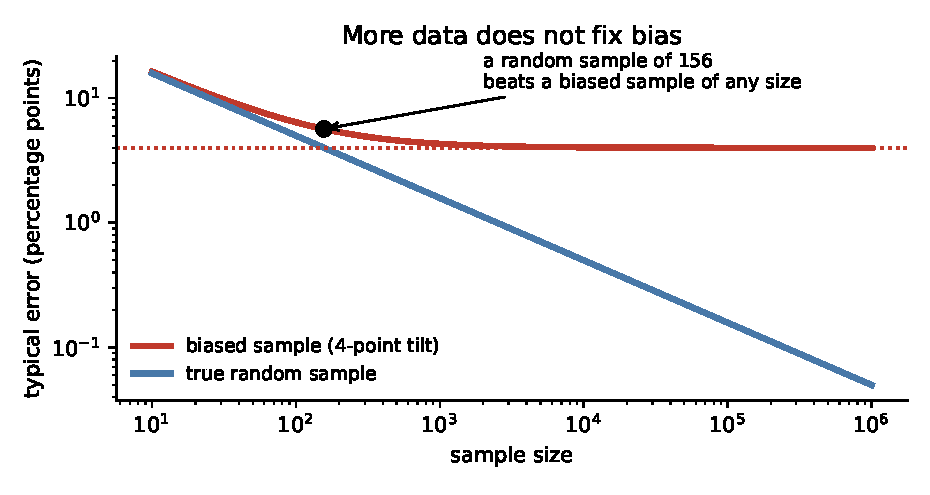
\includegraphics[width=\textwidth]{fig_m14_bias_vs_n.pdf}
\end{column}
\begin{column}{0.42\textwidth}
\small
A sample with a 4-point systematic tilt never gets more accurate than 4 points, however many rows
you add.
\begin{itemize}
  \item A \emph{random} sample of about \textbf{156} matches it.
  \item Worse: the huge sample reports a tiny standard error, so it is confidently wrong.
\end{itemize}
\end{column}
\end{columns}
\onslide<2->{\centering\small
This is exactly how 40 million app users can mislead you about your market.}
\end{frame}

\begin{frame}{Your turn \#1}
\begin{yourturn}{find the frame problem}
A streaming service estimates ``average weekly viewing hours per subscriber'' from telemetry sent
by its smart-TV app.
\vspace{0.3em}

With a neighbor: name three groups of subscribers this misses or distorts, and say which direction
the estimate is biased.
\end{yourturn}
\end{frame}

\begin{frame}{Your turn \#1: answer}
\begin{itemize}
  \item Subscribers who watch on phones, laptops, or game consoles are missing entirely, and their
        habits differ.
  \item Households sharing one account look like one heavy viewer, while a subscriber who never
        opens the app sends no telemetry at all and may vanish from the denominator.
  \item Anyone with telemetry disabled, or an older TV, is excluded, and both correlate with age
        and income.
\end{itemize}
\begin{principle}{ask what the instrument can see}
Telemetry measures device activity, not people watching. The gap between those two is where the
bias lives.
\end{principle}
\end{frame}

% ======================================================================
\section{Missing data}
% ======================================================================
\begin{frame}{Missing values in real data}
\begin{center}
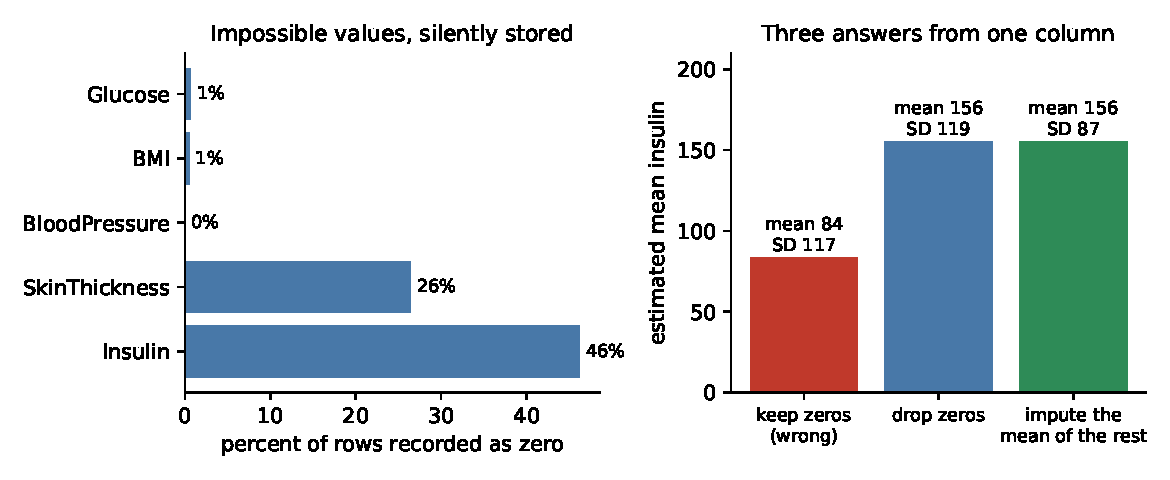
\includegraphics[width=0.92\textwidth]{fig_m14_missing.pdf}
\end{center}
\vspace{-0.4em}
\small
733 patients. Insulin is recorded as zero for \textbf{46\%} of them, which is biologically
impossible: those are missing values recorded as zero. Keeping them halves the estimated mean.
Mean imputation gets the mean right and shrinks the SD from 119 to 87, manufacturing precision that
does not exist.
\end{frame}

\begin{frame}{Three ways data goes missing}
\begin{itemize}
  \item \textbf{Missing completely at random:} the machine failed randomly. Dropping rows costs
        precision but is unbiased. Rare in practice.
  \item \textbf{Missing at random (given what you measured):} older patients skip a test more often,
        and you recorded age. Dropping is biased. Modeling with age is not.
  \item \textbf{Missing not at random:} the value itself drives the absence. High earners refuse to
        report income, and the sickest patients miss follow-up. Nothing in the data fixes this. You need
        external information or an explicit assumption.
\end{itemize}
\begin{trap}{silent listwise deletion}
Most software drops incomplete rows without telling you. If the dropped rows differ systematically,
your entire analysis quietly changed populations.
\end{trap}
\end{frame}

\begin{frame}{What to actually do}
\begin{enumerate}
  \item \textbf{Count and map the missingness} first, per column, and check whether missing rows
        differ from complete ones on the outcome.
  \item \textbf{Look for disguised codes}: 0, $-1$, 999, ``N/A'', or an empty string.
  \item \textbf{Add a missingness indicator} when absence itself might be informative. Often it is
        the most predictive feature you have.
  \item \textbf{Prefer multiple imputation} to single mean imputation, so the extra uncertainty
        shows up in the interval instead of vanishing.
  \item \textbf{Say what you did}, and show the result both ways.
\end{enumerate}
\end{frame}

% ======================================================================
\section{Measurement}
% ======================================================================
\begin{frame}{Weighting: the partial repair}
When your sample's composition is wrong but you \emph{know} the true composition, you can reweight.
\begin{center}\small
\begin{tabular}{lccc}
\toprule
\textbf{Age group} & \textbf{\% of population} & \textbf{\% of respondents} & \textbf{weight} \\
\midrule
18--34 & 30\% & 12\% & 2.50 \\
35--54 & 35\% & 33\% & 1.06 \\
55+    & 35\% & 55\% & 0.64 \\
\bottomrule
\end{tabular}
\end{center}
\vspace{0.4em}
\begin{itemize}
  \item Each young respondent now counts for 2.5 people, so the estimate reflects the population
        mix rather than who answered.
  \item It only fixes imbalance on variables you \emph{measured}, and heavy weights inflate the
        variance.
\end{itemize}
\begin{trap}{weighting as a blank check}
``We weighted the survey'' does not mean the bias is gone. It means the bias on the weighting
variables is gone.
\end{trap}
\end{frame}

\begin{frame}{Your turn \#3}
\begin{yourturn}{interrogate a dataset}
You are handed a dataset of loan applications that were \textbf{approved}, with a default
indicator, and asked to build a model deciding whom to approve next.
\vspace{0.3em}

With a neighbor: name the population this data actually represents, the group that is missing, and
the specific way a model trained on it would mislead the credit team.
\end{yourturn}
\end{frame}

\begin{frame}{Your turn \#3: answer}
\begin{itemize}
  \item The population is \textbf{applicants the old policy already approved}, not applicants in
        general. Everyone the previous rule rejected is invisible.
  \item The model therefore learns to reproduce the old policy's judgments, including its
        mistakes, and it has no information at all about the region of applicant space that was
        never approved.
  \item Consequence: it will look accurate in backtesting and will be unable to tell you whether
        the applicants you currently reject would in fact have repaid.
  \item Partial fixes: approve a small random sample of marginal applicants (deliberate
        exploration), or use the rejected applicants' outcomes elsewhere if they can be observed.
\end{itemize}
\end{frame}

\begin{frame}{You measure a proxy, not the concept}
\begin{itemize}
  \item ``Engagement'' becomes clicks. ``Teacher quality'' becomes test scores. ``Customer
        happiness'' becomes a survey score from the 6\% who responded.
  \item Every proxy has a gap between it and the real concept, and decisions get made in that gap.
  \item \textbf{Goodhart's law:} once a proxy becomes a target, people optimize the proxy, and the
        gap widens on purpose.
\end{itemize}
\begin{practice}{a strong thing to raise unprompted}
``Before I model this, what exactly does this column measure, who recorded it, and when? Half the
projects I have seen went wrong at that step.''
\end{practice}
\end{frame}

\begin{frame}{Measurement problems that look like findings}
\begin{itemize}
  \item \textbf{Instrument drift:} a logging change in March makes April look like a behavior shift.
  \item \textbf{Question wording:} ``Do you support banning X?'' and ``Do you oppose allowing X?''
        give different numbers from identical people.
  \item \textbf{Social desirability:} people over-report voting, exercise, and reading. They
        under-report drinking and screen time.
  \item \textbf{Definition changes:} a churn spike caused by moving the churn cutoff from 90 to 60
        days.
\end{itemize}
\begin{trap}{check the instrument before the world}
Before explaining a sudden jump with a story about the world, check whether the instrument changed
on that date. It usually did.
\end{trap}
\end{frame}

\begin{frame}{Your turn \#2}
\begin{yourturn}{whose data is it?}
A hiring team builds a model to predict "good employees" using performance ratings from the past
ten years of hires.
\vspace{0.3em}

With a neighbor: identify one selection problem, one measurement problem, and one missing-data
problem in that setup.
\end{yourturn}
\end{frame}

\begin{frame}{Your turn \#2: answer}
\begin{itemize}
  \item \textbf{Selection:} you only observe performance for people who were \emph{hired}. Rejected
        candidates who would have excelled are invisible, so the model learns the old process's
        preferences.
  \item \textbf{Measurement:} ``performance rating'' is a manager's judgment, carrying whatever
        biases and grade inflation that manager had. It is a proxy, not the concept.
  \item \textbf{Missing:} people who left early have no rating, and they left for reasons related
        to the outcome. That is missing not at random.
\end{itemize}
\begin{principle}{the model inherits the process that made the data}
A model trained on past decisions predicts the past decisions, including their mistakes. That is
not a bug you can regularize away.
\end{principle}
\end{frame}

% ======================================================================
\section{LLM check}
% ======================================================================
\begin{frame}{LLM check: mistake or not? (1 of 2)}
\begin{llmcheck}{we asked an LLM about sample size}
\textbf{We told it:} ``Our survey of app users got 40,000 responses out of 2 million invitations.
Is that enough to represent our user base?''\\[4pt]
\textbf{It answered:} ``Yes, 40,000 is an excellent sample size. The margin of error is under 0.5\%,
so you can be very confident these results represent your users.''
\end{llmcheck}
\vspace{0.2em}
\centering\small Mistake, or no mistake?
\onslide<2->{%
\begin{trap}{verdict: mistake}
A 2\% response rate is the headline, not the 40{,}000. The margin of error describes sampling
error only, and says nothing about the 98\% who did not answer. The tiny stated error makes the
result more dangerous, not more trustworthy.
\end{trap}}
\end{frame}

\begin{frame}{LLM check: mistake or not? (2 of 2)}
\begin{llmcheck}{same territory, a different answer}
\textbf{We told it:} ``Our dataset has 30\% missing income values. Should I fill them with the
median?''\\[4pt]
\textbf{It answered:} ``First check whether the missingness is related to income itself, since high
earners often decline to report. If so, median imputation will bias your estimates downward and
also understate your uncertainty. I would add a missing-indicator, use multiple imputation, and
report results with and without the imputed rows.''
\end{llmcheck}
\vspace{0.2em}
\centering\small Mistake, or no mistake?
\onslide<2->{%
\begin{principle}{verdict: no mistake}
It diagnosed the missingness mechanism before choosing a repair, and it flagged the understated
uncertainty that single imputation causes.
\end{principle}}
\end{frame}

% ======================================================================
\section{Workflow}
% ======================================================================
\begin{frame}{The questions to ask before you model}
\begin{enumerate}
  \item \textbf{What population} does this decision concern?
  \item \textbf{What frame} produced these rows, and who is in the gap?
  \item \textbf{Who is missing because of the outcome} we are studying?
  \item \textbf{What does each column really measure}, who recorded it, and when?
  \item \textbf{Where are the missing values}, how are they coded, and do those rows differ?
  \item \textbf{What changed over time} in the instrument, the definition, or the pipeline?
  \item \textbf{What could I not fix}, and how do I state it in the writeup?
\end{enumerate}
\end{frame}

\begin{frame}{Scenario: the customer survey that ended a product}
\textbf{Setup.} A satisfaction survey emailed to all users returns 4\% response and an average of
3.1 out of 5. Leadership plans to kill the feature.
\begin{itemize}
  \item The 4\% who answered are disproportionately the annoyed and the delighted. The score is a
        mixture of two tails, not a measure of the middle.
  \item Better evidence: behavioral data on all users (does usage predict retention?), or a
        \emph{random} subsample contacted persistently until you get a high response rate from
        those specific people.
  \item Cheap check: compare responders and non-responders on the variables you \emph{do} have.
        If they differ on tenure and usage, they differ on satisfaction too.
\end{itemize}
\begin{interview}{how to answer}
``The 3.1 describes responders. Before acting I would compare responders to non-responders and get
behavioral evidence from the full base.''
\end{interview}
\end{frame}

% ======================================================================
\section{Consolidate}
% ======================================================================
\begin{frame}{The audit to run before you model anything}
\small
\begin{enumerate}
  \item \textbf{Name the population} the decision concerns, and the frame the rows actually came from.
  \item \textbf{Ask who is missing because of the outcome} you are studying.
  \item \textbf{Count the missing values per column}, and look for them in disguise: 0, $-1$, 999, empty strings.
  \item \textbf{Compare rows with missing values to complete rows} on the outcome. If they differ, dropping them changes the population.
  \item \textbf{Ask what each column really measures}, who recorded it, and when.
  \item \textbf{Check for breaks over time} in the instrument, the definition, or the pipeline.
  \item \textbf{Write down what you could not fix}, and put it in the report.
\end{enumerate}
\end{frame}

\begin{frame}{The traps, all in one place}
\begin{trap}{the ones that bite most often}
\begin{itemize}
  \item Treating a big sample as a representative one.
  \item Studying only survivors, winners, or responders.
  \item Reporting a margin of error that ignores nonresponse.
  \item Dropping incomplete rows without checking how they differ.
  \item Mean-imputing and then quoting the tighter interval.
  \item Analyzing clustered data as if rows were independent.
  \item Forgetting that a proxy is not the concept, especially once it becomes a target.
\end{itemize}
\end{trap}
\end{frame}

\begin{frame}{Ten questions to be able to answer}
\begin{enumerate}\small
  \item We have 40 million records. Is that representative?
  \item Our response rate was 8\%. What can we conclude?
  \item Explain survivorship bias with an example from business.
  \item What do you do about missing values, and what do you check first?
  \item What is the difference between undercoverage and nonresponse?
  \item When would a sample of 1{,}000 beat a sample of 10 million?
  \item How would you design a sample to estimate this on a fixed budget?
  \item Our metric jumped on March 3. What do you check before explaining it?
  \item What is the risk of using clicks as a proxy for engagement?
  \item Why can a model trained on past hiring decisions be unfair with no protected attributes?
\end{enumerate}
\end{frame}

\begin{frame}{Mastery checklist}
You have this unit when you can, from memory:
\begin{itemize}
  \item distinguish population, frame, and sample, and locate the bias at each step
  \item choose among simple, stratified, cluster, and systematic designs
  \item recognize survivorship and nonresponse bias in a described study
  \item explain why bias does not shrink with sample size
  \item classify missingness and choose a defensible repair
  \item critique a measurement as a proxy for the concept it stands in for
\end{itemize}
\end{frame}

\begin{frame}{What you should be able to do with software}
\small
Nobody is asking you to memorize syntax. You are expected to know \emph{which} procedure the
question calls for, what to hand it, and what the output means. With an AI assistant open, you
should be able to produce any of these and defend the result.
\begin{center}\footnotesize
\begin{tabular}{p{0.44\textwidth} p{0.46\textwidth}}
\toprule
\textbf{You should be able to} & \textbf{What you would reach for} \\
\midrule
Missingness by column & \texttt{df.isna().sum()}, and \texttt{(df[col] == 0).mean()} \\
Compare responders to non-responders & \texttt{groupby} on a missingness indicator \\
A missing-value indicator as a feature & \texttt{df[\"x\_missing\"] = df.x.isna().astype(int)} \\
Multiple imputation rather than the mean & \texttt{sklearn.impute.IterativeImputer} \\
Stratified and cluster sampling & \texttt{groupby(...).sample} \\
Reweight to a known population mix & weights = population share / sample share \\
Cluster-aware standard errors & resample the cluster, not the row \\
\bottomrule
\end{tabular}
\end{center}
\vspace{0.2em}
\centering\small
If you cannot say what the output means, the fact that you produced it is worth nothing.
\end{frame}

\begin{frame}{Where we go next}
\begin{itemize}
  \item That closes Part I. Five units of building models and one on whether the data underneath
        them deserved the trust.
  \item Sampling raised a question we have been dodging since Unit 1: what does \emph{random}
        actually mean, and how do we compute with it?
  \item \textbf{Part II} answers it. Unit 7 does probability, Unit 8 puts numbers on uncertain
        outcomes, and \textbf{Unit 9} finally proves the result every standard error in Part I was
        quietly assuming.
\end{itemize}
\begin{principle}{the habit to keep}
The most important question in any analysis comes before the first line of code: where did this
data come from, and who is not in it?
\end{principle}
\end{frame}

\end{document}
